\documentclass[12pt,a4paper]{article}
\usepackage{amsmath,amscd,amsbsy,amssymb,latexsym,url,bm,amsthm}
\usepackage{epsfig,graphicx,subfigure}
\usepackage{enumitem,balance}
\usepackage{wrapfig}
\usepackage{mathrsfs,euscript}
\usepackage[usenames]{xcolor}
\usepackage{hyperref}
\usepackage[vlined,ruled,linesnumbered]{algorithm2e}
\hypersetup{colorlinks=true,linkcolor=black}

\newtheorem{theorem}{Theorem}
\newtheorem{lemma}[theorem]{Lemma}
\newtheorem{proposition}[theorem]{Proposition}
\newtheorem{corollary}[theorem]{Corollary}
\newtheorem{exercise}{Exercise}
\newtheorem*{solution}{Solution}
\newtheorem{definition}{Definition}
\theoremstyle{definition}

\renewcommand{\thefootnote}{\fnsymbol{footnote}}

\newcommand{\postscript}[2]
 {\setlength{\epsfxsize}{#2\hsize}
  \centerline{\epsfbox{#1}}}

\renewcommand{\baselinestretch}{1.0}

\setlength{\oddsidemargin}{-0.365in}
\setlength{\evensidemargin}{-0.365in}
\setlength{\topmargin}{-0.3in}
\setlength{\headheight}{0in}
\setlength{\headsep}{0in}
\setlength{\textheight}{10.1in}
\setlength{\textwidth}{7in}
\makeatletter \renewenvironment{proof}[1][Proof] {\par\pushQED{\qed}\normalfont\topsep6\p@\@plus6\p@\relax\trivlist\item[\hskip\labelsep\bfseries#1\@addpunct{.}]\ignorespaces}{\popQED\endtrivlist\@endpefalse} \makeatother
\makeatletter
\renewenvironment{solution}[1][Solution] {\par\pushQED{\qed}\normalfont\topsep6\p@\@plus6\p@\relax\trivlist\item[\hskip\labelsep\bfseries#1\@addpunct{.}]\ignorespaces}{\popQED\endtrivlist\@endpefalse} \makeatother

\begin{document}
\noindent

%========================================================================
\noindent\framebox[\linewidth]{\shortstack[c]{
\Large{\textbf{Lab05-Graph Algorithm}}\vspace{1mm}\\
Algorithm and Complexity, Xiaofeng Gao, Spring 2022.}}
\begin{center}
\footnotesize{\color{red}$*$ If there is any problem, please contact TA Jialin Lyu.}

% Please write down your name, student id and email.
\footnotesize{\color{blue}$*$ Name: Zhenran Xiao  \quad Student ID: 520030910281 \quad Email: xiaozhenran@sjtu.edu.cn}
\end{center}



\begin{enumerate}
    \item
    Given an undirected graph $G = (V, E)$ in Figure \ref{Fig-1}, supposed that vertices are numbered from $A$ to $L$, please complete the following tasks:

	\begin{figure}[!htbp]
	\centering
	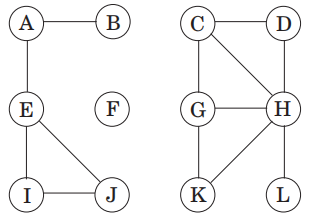
\includegraphics[width=0.4\textwidth]{Fig-1.png}
	\caption{A sample of undirected graph.}
	\label{Fig-1}
	\end{figure}

    \begin{enumerate}
        \item
        Please use DFS and BFS respectively to establish all the connected components. It is assumed that always start from the vertex with the smallest lexicographic order and visit its adjacent vertices in order of increasing lexicographic order.
        \item
        According to question (a), both DFS and BFS yield a tree (also possibly forest), please draft the tree and list all the tree, forward, back and cross edges (if there exists) respectively for DFS and BFS. Moreover, please list PREVISIT and POSTVISIT interval $[pre(v), post(v)]$ for each vertex $v$ in DFS.
    \end{enumerate}

    \begin{solution}
    	\quad \\
    	\begin{enumerate}
   		\item There are three connected components established by DFS: \\
   		
   		\begin{figure}[!htbp]
   			\centering
   			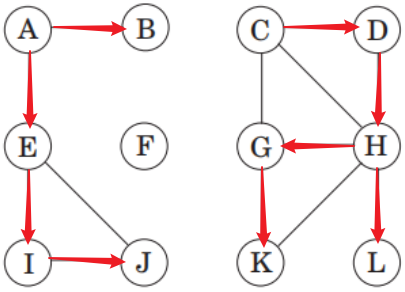
\includegraphics[width=0.4\textwidth]{Q1a-1.png}
   			\caption{Connected componets established by DFS}
   			\label{Fig-Q1a-1}
   		\end{figure}
   		
   		There are three connected components established by BFS: \\
   		
   		\begin{figure}[!htbp]
   			\centering
   			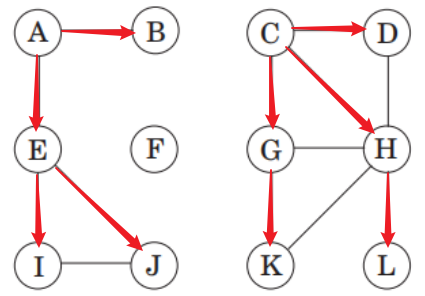
\includegraphics[width=0.4\textwidth]{Q1a-2.png}
   			\caption{Connected componets established by BFS}
   			\label{Fig-Q1a-2}
   		\end{figure}
   		
   		\item The forest yielded by DFS with root A, root C and root F. \\
   		
   		\begin{figure}[!htbp]
   			\centering
   			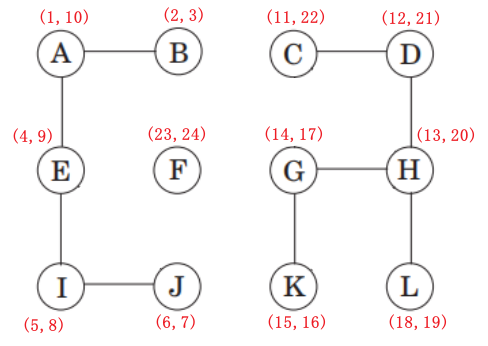
\includegraphics[width=0.4\textwidth]{Q1b-1.png}
   			\caption{Forest yielded by DFS}
   			\label{Fig-Q1b-1}
   		\end{figure}
   	
   		Forward edges: (A,I),(A,J),(E,J),(C,H),(C,G),(C,L),(C,K),(D,G),(D,L),(D,K),(H,K) \\
   		Back edges: 
   		(I,A),(J,A),(J,E),(H,C),(G,C),(L,C),(K,C),(G,D),(L,D),(K,D),(K,H) \\
   		Cross edges: 
		(E,B),(I,B),(J,B),(L,K),(L,G), and edges from F to all the other vertexes. \\
		
		The forest yielded by BFS with root A, root C and root F. \\
		
		\begin{figure}[!htbp]
			\centering
			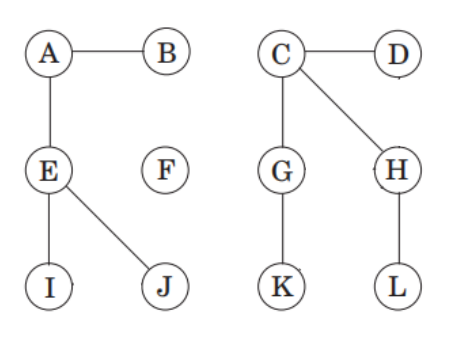
\includegraphics[width=0.4\textwidth]{Q1b-2.png}
			\caption{Forest yielded by BFS}
			\label{Fig-Q1b-2}
		\end{figure}
		
		Forward edges: (A,I),(A,J),(C,K),(C,L) \\
		Back edges: (I,A),(J,A),(K,C),(L,C)\\
		Cross edges: (E,B),(J,I),(I,B),(J,B),(G,D),(H,D),(L,K),(L,G), and edges from F to all the other vertexes. \\
		
    	\end{enumerate}
    \end{solution}

    \item
    In addition to edge capacities, a flow network has vertex capacities. That is each vertex has a limit on how much flow can pass though. Show how to transform a flow network $G = (V, E)$ with vertex capacities into an equivalent flow network $G' = (V ', E')$ without vertex capacities, such that a maximum flow in $G'$ has the same value as a maximum flow in $G$. How many vertices and edges does $G'$ have? (An illustrative example is shown in Figure \ref{Fig-2}, you may give the solution of Figure \ref{Fig-2} first, and then give the general solution.)

    \begin{figure}[!htbp]
	\centering
	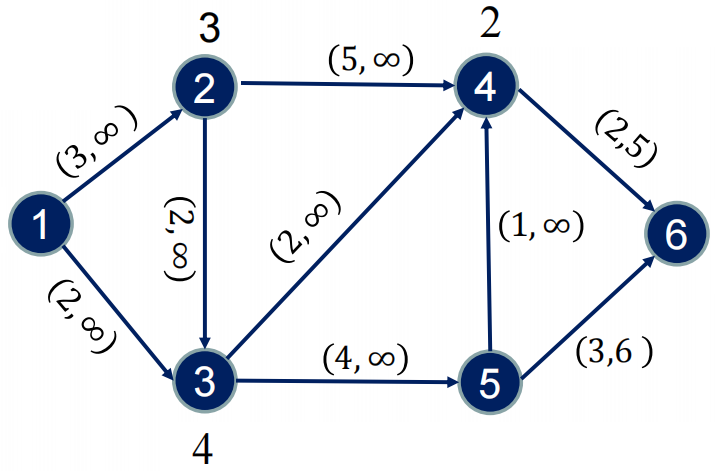
\includegraphics[width=0.4\textwidth]{Fig-2.png}
	\caption{A sample of flow network with vertex capacities. (The number adjacent to each vertex represents the vertex capacity. The first item of each directed edge represents its value, and the second item represents its edge capacity.)}
	\label{Fig-2}
	\end{figure}

    \begin{solution}
        \quad \\
        Transforming method: divide a vertex $m$ with vertex capacity into two vertices $u$ and $v$ without vertex capacity; add an edge from $u$ to $v$ with edge capacity equal to the original vertex capacity; let the original edges that flow into vertex $m$ flow into $u$, and the original edges that flow out from $m$ flow out from $v$. \\
        
        \begin{figure}[!htbp]
           	\centering
           	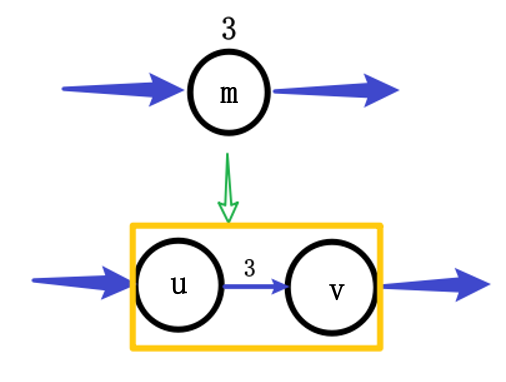
\includegraphics[width=0.4\textwidth]{Q2-1.png}
           	\caption{The image of transforming method}
           	\label{Fig-Q2-1}
        \end{figure}
    
    	So the equivalent flow network of the network in Figure \ref{Fig-2} is: 
    	\begin{figure}[!htbp]
    		\centering
    		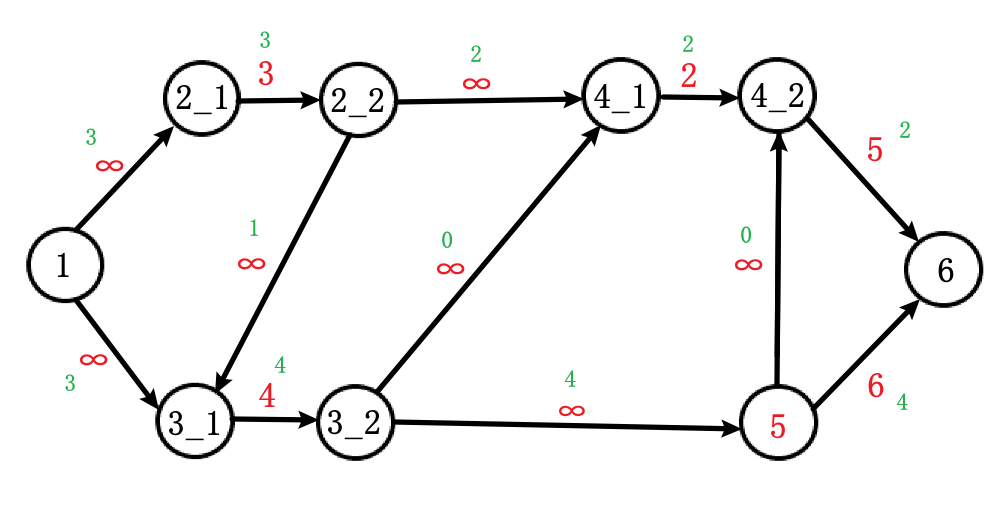
\includegraphics[width=0.6\textwidth]{Q2-2.png}
    		\caption{The equivalent flow network of the network in Figure \ref{Fig-2}}
    		\label{Fig-Q2-2}
    	\end{figure}
    
    \end{solution}

You can choose one of the following questions (Question $3$ and Question $4$) to answer. You will get extra bonus points if you finish both of them correctly. Otherwise, you will get the highest score among them.

    \item
    \textit{Information Transmission.} During a war, the information from different regions in a country can be transmitting by the following $2$ sending modes:
    \begin{itemize}
    \item \textbf{Telegram mail mode:} If city $A$ has the conditions to transmit telegram to city $B$, then city $A$ can transmit telegram to city $B$ \textbf{in one direction} at a certain time. (The unit of time is minute, and the time required is not necessarily the same if it is transmitted in the opposite direction.) In addition, if the telegram can't be transmitted directly, city $A$ can also transmit telegram to other cities, then other cities maybe have the conditions to transmit it to the city $B$;
    \item \textbf{Internet transmission mode:} If both city $A$ and city $B$ can send telegram to each other (telegram sent from any one of the cities can be delivered to the other one, and it is allowed to transmit information passing through other cities), it can be considered that city $A$ and city $B$ are in the same region. In that case, the two cities $A$ and $B$ can transmit information to each other through the Internet immediately and without spending any extra time;
    \end{itemize}

    Given the required time of sending telegram between different cities in the country, please help to calculate the minimum time to send information between different cities or to tell that the message cannot be transmitted.

    \textbf{Input Specification:}

    There are multiple test cases. The first line of the input is an integer $T (1 \leq T \leq 10)$, indicating the number of test cases. Then $T$ test cases follow.

    The first line of each test case contains two integer separated by a space, $N (1 \leq N \leq 500)$ and $E (0 \leq E \leq N^2)$, indicating the number of cities (numbered from $1$ to $N$) and the number of agreements on sending telegrams, respectively.

    Then $E$ lines follows, each line contains three integers separated by spaces, $X, Y, M (1 \leq X, Y \leq N, 1 \leq M \leq 1000)$, indicating that there exist an agreement to send a telegram from city $X$ to city $Y$, and that such a telegram will be delivered in $M$ minutes.

    After that, there will be a line with an integer $K (0 \leq K \leq 100)$, the number of queries.

    Finally, there will be $K$ lines, each representing a query and containing two integers separated by a space, $A, B (1 \leq A, B \leq N)$. You must determine the minimum time to send information from city $A$ to city $B$.

    \textbf{Output Specification:}

    For each test case output $K$ lines. The $i$-th line should contain an integer, indicating the minimum time (in minutes) of sending telegram of the $i$-th query. If there aren��t communication conditions between the cities of the query, print ��Impossible�� (without quotes) in one line instead.

    \fbox{
    \begin{minipage}[t]{0.2\textwidth}
    \textbf{Sample Input:}
	
	2 \\ 4 5 \\ 1 2 5 \\ 2 1 10 \\ 2 3 6 \\ 3 4 8 \\ 4 3 7 \\ 5 \\ 1 2 \\ 1 3 \\ 1 4 \\ 4 3 \\ 4 1 \\ 3 3 \\ 1 2 10 \\ 2 3 1 \\ 3 2 1 \\ 3 \\ 1 3 \\ 3 1 \\ 3 2
    \end{minipage}
    \begin{minipage}[t]{0.2\textwidth}
    \textbf{Sample Output: }
	
	0 \\ 6 \\ 6 \\ 0 \\ Impossible \\ 10 \\ Impossible \\ 0
    \end{minipage}}
    \hspace{1cm}
    \begin{minipage}[t]{0.45\textwidth}
    \textbf{Remark:} The input data \texttt{Lab05-Telegram.in} (sample test cases only) and the template code \texttt{Lab05-Telegram.cpp} are attached on the course webpage. Please include your \texttt{Lab05-Telegram.cpp} file in your uploaded .rar or .zip file.
    \end{minipage}

    \begin{enumerate}
    \item
    Please briefly describe your algorithm and analyze its time complexity and space complexity.

    \item
    Try to write a C/C++ code to solve this problem, you only need to complete the \texttt{TODO} part in \texttt{Lab05-Telegram.cpp}. Your program will be judged by the online judge system, including several test cases, half for the test data which equivalent to the sample test case, and another half for other corner and huge test cases.
    \end{enumerate}

    \begin{solution}
    	\quad \\
        \begin{enumerate}
        \item For every query City A to City B, use Floyd-Warshall Alogrithm twice to find the shortest sending time from A to B and from B to A. If both the two path exist, the actual sending time is 0(by Internet). If only the path from A to B exists, the sending time is the path. If the path from A to B doesn't exist, it is impossible to mail between the two cities. \\
        The time complexity: $O(N^3)$ \\
        The space complexity: $O(N^2)$ \\
        
        \item Please check it in \texttt{Lab05-Telegram.cpp}. \\
        
        \begin{figure}[!htbp]
        	\centering
        	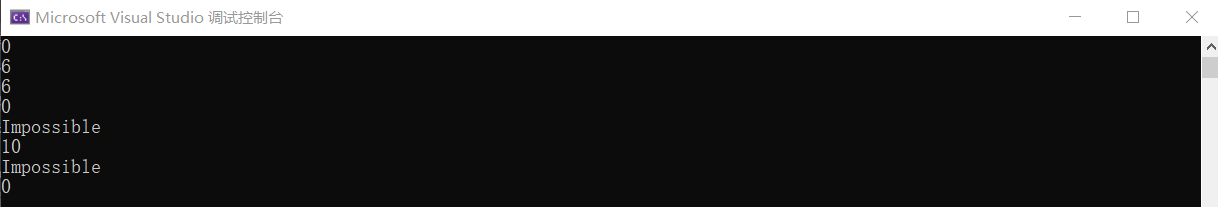
\includegraphics[width=0.87\textwidth]{Q3b.png}
        	\caption{Output of Lab05-Telegram.cpp}
        	\label{Fig-Q3b}
        \end{figure}
        
        \end{enumerate}
    	
    \end{solution}

    \item
    \textit{Punch in Shanghai Metro.} Little Gyro is a subway fan. This holiday he finally has the opportunity to come to Shanghai ���� the capital of the subway, and want to have fun in taking subway.

    The pricing rule of Shanghai Metro is that the starting price is $3$ yuan, and the shortest distance between the departure station and the arrival station is increased by $1$ yuan per $K$ kilometers.

    For example, let $K = 10$, Hongqiao Railway Station is $20$ kilometers away from People's Square Station, so that the fare between them is $3 + 2 = 5$ yuan.

    In order to get the greatest satisfaction, Little Gyro decides to take the subway in the following way: If Little Gyro gets on at a certain station (set it as subway station $A$), for all arrival stations with the same fare, Little Gyro will only exit at the station with the farthest distance or terminal, take a punch photo outside the station, and then take subway to the next station in the same way.

    Given the departure station (Little Gyro would also take a punch card photo before setting out), while taking the subway, Little Gyro suddenly becomes curious about how many punch photos at most and at which subway stations could he take during the whole journey.

    \textbf{Hint:} Subway refers to the urban traffic rail system which mainly runs underground. Generally speaking, the subway is composed of several stations and many different lines running in both directions.

    When two or more lines pass through the same station, you can transfer and change the line you take. For example, both Line $1$ and Line $2$ of the Shanghai Metro pass through the People's Square Station, then when you arrive at the People's Square by Line $1$, you can transfer to Line $2$ to go to various stations of Line $2$. In that case, you needn't to exit the station for transfer (Outbound transfer is not considered), so that you can't get a punch photo at the same time. As a result, there are no restrictions on transfer while Little Gyro taking the subway.

    \begin{figure}[!htbp]
	\centering
	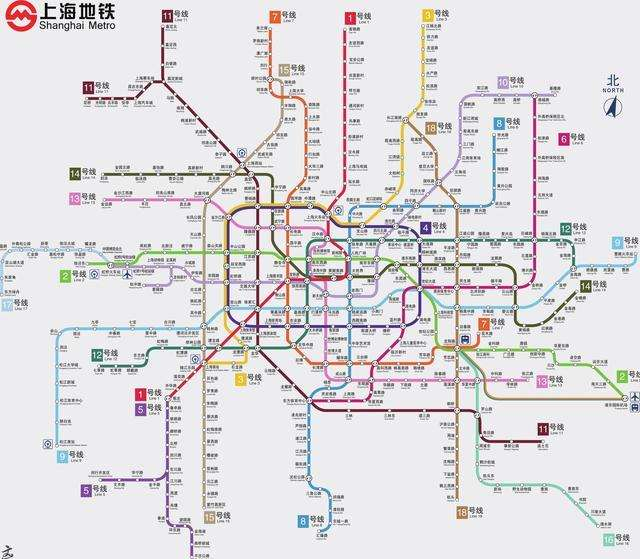
\includegraphics[width=0.7\textwidth]{Fig-3.jpeg}
	\caption{The map of Shanghai Metro.}
	\label{Fig-3}
	\end{figure}

    \textbf{Input Specification:}

    There are multiple test cases. The first line of the input is an integer $T (1 \leq T \leq 10)$, indicating the number of test cases. Then $T$ test cases follow.

    The first line of each test case contains three integers $N, M, K (1 \leq N \leq 200, 1 \leq M \leq 1500, 1 \leq K \leq 10^6)$, indicating the number of stations, the number of lines of Shanghai Metro, and increase the fare by $1$ yuan per $K$ kilometers, respectively.

    The following $M$ lines describe the information of Shanghai Metro lines, with the following format:

    $<Station 1><Space><Distance><Space><Station 2><Space><Distance><Space><Station 3> \dots <Station (X-1)><Space><Distance><Space><Station X>$

    Where $<Station X>$ is a number from $1$ to $N$. $<Distance>$ between two station numbers $<Station (X-1)>, <Station X>$ refers to the distance of two stations on the line. The distance between two stations is a positive integer not greater than $10^6$. The stations on each line are unique.

    \textbf{Hint:} It maybe exists multiple directly connected lines between two subway stations, and the distances between them are not necessarily equal.

    After that, there will be a line with an integer $Q (0 \leq Q \leq 200)$, the number of queries of the departure subway stations.

    Finally, there will be $Q$ lines, each representing a query and containing one integer $X_i (1 \leq X_i \leq N)$, indicating the departure subway station that Little Gyro choose.

    \textbf{Output Specification:}

    For each query output two lines, the first line consists one integer, indicating the maximum number of punch photos that Little Gyro could take. The second line consists several numbers, indicating the station number (within the ascending order) that Little Gyro could punch in.

    Please, \textbf{DO NOT} output extra spaces at the end of each line, or your program may be considered incorrect!

    \fbox{
    \begin{minipage}[t]{0.2\textwidth}
    \textbf{Sample Input:}
	
	2 \\ 6 2 6 \\ 5 6 2 6 6 \\ 1 6 2 4 3 1 4 \\ 4 \\ 5 \\ 4 \\ 3 \\ 2 \\ 6 2 6 \\ 1 1 2 1 3 \\ 4 2 5 2 6 \\ 4 \\ 1 \\ 5 \\ 4 \\ 2
    \end{minipage}
    \begin{minipage}[t]{0.2\textwidth}
    \textbf{Sample Output: }
	
	5 \\ 1 2 4 5 6 \\ 5 \\ 1 2 4 5 6 \\ 6 \\ 1 2 3 4 5 6 \\ 5 \\ 1 2 4 5 6 \\ 2 \\ 1 3 \\ 3 \\ 4 5 6 \\ 2 \\ 4 6 \\ 3 \\ 1 2 3
    \end{minipage}}
    \hspace{1cm}
    \begin{minipage}[t]{0.45\textwidth}
    \textbf{Remark:} The input data \texttt{Lab05-SHMetro.in} (sample test cases only) and the template code \texttt{Lab05-SHMetro.cpp} are attached on the course webpage. Please include your \texttt{Lab05-SHMetro.cpp} file in your uploaded .rar or .zip file.
    \end{minipage}

	\begin{enumerate}
    \item
    Please briefly describe your algorithm and analyze its time complexity and space complexity.

    \item
    Try to write a C/C++ code to solve this problem, you only need to complete the \texttt{TODO} part in \texttt{Lab05-SHMetro.cpp}. Your program will be judged by the online judge system, including several test cases, half for the test data which equivalent to the sample test case, and another half for other corner and huge test cases.
    \end{enumerate}

%    \begin{solution}
%        Uncomment this block to write your solution.
%    \end{solution}

\end{enumerate}

\vspace{20pt}

\textbf{Remark:} You need to include your .pdf and .tex files in your uploaded .rar or .zip file.

%========================================================================
\end{document}
